\subsection{Reading a near miss and a false positive from their band edges}
The band-edge thresholds and gap window test different properties. Figure~\ref{fig:bands} compares the contest's two reported edges with their cutoffs and places the modeled and public gaps for $\mathrm{CaZrO_3}$ on a separate axis.

\begin{figure}[htbp]
\centering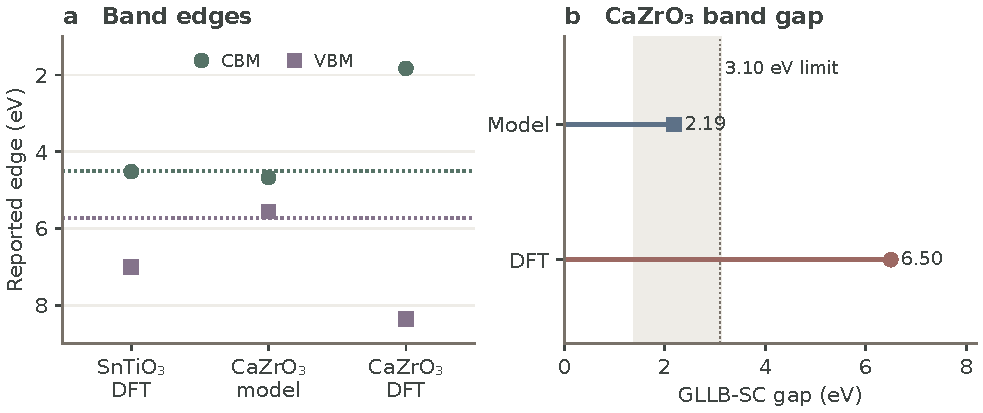
\includegraphics[width=\linewidth]{figures/band_edges.pdf}
\caption{Public DFT values and seed-26 property-model estimates. Left, the dotted lines mark the CBM (4.50 eV) and VBM (5.73 eV) cutoffs on the contest's inverted edge axis. Right, shading marks the 1.40--3.10 eV accepted gap interval.}\label{fig:bands}
\end{figure}

For $\mathrm{SnTiO_3}$, the CBM lies 0.018833 eV beyond its cutoff, a difference too small to resolve easily at the figure scale. For $\mathrm{CaZrO_3}$ the observed edges both pass, but the observed gap is 6.50 eV. It exceeds the upper limit by 3.40 eV and produces the entire observed violation of 46.24.

The modeled band edges help explain how the four-property model can rank that material first. It predicts $g=2.1883$ eV, with both small band-edge violations and a passing formation energy, for a total predicted $V=0.2342$. Its independently fitted edges imply $5.5559-4.6680=0.8879$ eV, far from its own gap estimate. In the public DFT record the analogous difference is 6.53 eV, close to the tabulated 6.50 eV. The discrepancy between the model's two estimates of the gap provides a composition-level warning that could be checked before spending a single assay. The following sensitivity test evaluates this warning across all Q3 validation pairs.

\subsection{Can a consistency check rescue a one-choice screen?}
The $\mathrm{CaZrO_3}$ failure suggests a testable diagnostic. Define
\[
 D(z)=\big|\hat g(z)-(\hat v(z)-\hat c(z))\big|.
\]
All three terms are predictions from the property-first model, so the diagnostic could be computed before measuring a candidate. It checks whether the two representations of the gap agree. A small residual can also occur when both representations are wrong in the same direction.

We test a veto on the 1,701 Q3 validation records. We discard predictions with $D>\tau$ and select the remaining candidate with the smallest property-first violation. Table~\ref{tab:veto} reports both seeds, with 26 first in each entry. The same 11 near-targets are available to each fit. Thresholds are exploratory, and this test does not alter the frozen mixture.
\begin{table}[htbp]
\caption{Cost of vetoing inconsistent property predictions. Entries give seed 26 / seed 42. Counts refer to distinct Q3 validation records.}\label{tab:veto}
\centering\small\begin{tabular}{lrrr}
\toprule Tolerance (eV) & Eligible records & Near-targets retained & First observed $V$\\\midrule
No veto & 1701 / 1701 & 11 / 11 & 46.24 / 46.24\\
1.00 & 1698 / 1699 & 11 / 10 & 11.25 / 46.24\\
0.50 & 1690 / 1681 & 10 / 9 & 11.97 / 11.25\\
0.25 & 1634 / 1623 & 7 / 5 & 11.97 / 10.88\\
0.05 & 753 / 805 & 0 / 3 & 10.88 / 10.93\\\bottomrule
\end{tabular}
\end{table}

At $\tau=0.50$ the large error on $\mathrm{CaZrO_3}$ is removed for both seeds, yet neither replacement is a near-target. At $\tau=0.05$ the seed-26 screen eliminates every available near-target. Agreement between model outputs can flag a case for inspection. Using that agreement as an automatic rejection criterion sacrifices some of the materials the screen is meant to find.

